\date{}
\title{}
\date{}
\begin{document}
\begin{frame}
    \titlepage
\end{frame}

\section{IP addresses}

\subsection{IPv4}

\subsubsection{address format}
\begin{frame}{IPv4 addresses}
    \begin{itemize}
    \item 32-bit numbers
    \item typically written like 128.143.67.11
        \begin{itemize}
        \item four 8-bit decimal values separated by dots
        \item first part is most significant
        \item same as $128\cdot 256^3+143\cdot 256^2 + 67\cdot256 + 11 = 2\,156\,782\,459$
        \end{itemize}
    \end{itemize}
\end{frame}


\subsubsection{CIDR notation}
\begin{frame}{IPv4 address blocks}
\begin{itemize}
    \item often will want to talk about group of IPv4 addresses
    \item example: {\color<2>{violet!70!black}128.143.67.64}---{\color<2>{green!70!black}128.143.67.127} (inclusive)
    \item<2-> {\tt\color<2>{violet!70!black}\myemph<3>{10000000 10001111 01000011 001}\myemph<4>{00000}}
    \item<2-> {\tt\color<2>{green!70!black}\myemph<3>{10000000 10001111 01000011 001}\myemph<4>{11111}}
    \item<3-> first 27 bits always same; anything for last bits
    \item<5-> more convenient representation: 128.143.67.64/27
    \item<5-> called ``CIDR notation''
        \begin{itemize}
        \item CIDR = classless inter-domain routing (will come up when we discuss routing)
        \end{itemize}
\end{itemize}
\end{frame}

\begin{frame}{CIDR notation examples}
    \begin{itemize}
    \item 5.7.3.3/14 = 5.4.0.0/14 = 5.4.0.0---5.7.255.255
        \begin{itemize}
        \item<2-> \myemph<2>{also written 5.4/14}
        \end{itemize}
    \item 128.143.0.0/16 =  128.143.0.0---128.143.255.255
        \begin{itemize}
        \item<2-> \myemph<2>{also written 128.143/16}
        \end{itemize}
    \item 192.168.0.0/24 =  192.168.0.0---192.168.0.255
    \item 10.0.0.0/8 = 10.0.0.0--10.255.255.255
        \begin{itemize}
        \item<2-> \myemph<2>{also written 10/8}
        \end{itemize}
    \end{itemize}
\end{frame}

\begin{frame}{alternate notation: netmasks}
    \begin{itemize}
    \item instead of writing 128.143.67.64/27 might say
    \item 128.143.67.64 and ``network mask'' of 255.255.255.224
    \item 255.255.255.224 = 27 1's
    \vspace{.5cm}
    \item<2-> if some-address bitwise-AND netmask = 128.143.67.64 bitwise-AND netmask, \\
        then some-address is in the range
    \end{itemize}
\end{frame}


\subsection{IPv6}
\begin{frame}{IPv6 addresses}
    \begin{itemize}
    \item IPv6 like IPv4, but with 128-bit numbers
    \item written in hex, 16-bit parts, seperated by colons (\texttt{:})
    \item strings of 0s represented by double-colons (\texttt{::})
    \item typically given to users in blocks of $2^{80}$ or $2^{64}$ addresses
    \vspace{.5cm}
    \item \fontsize{10}{11}\selectfont\texttt{2607:f8b0:400d:c00::6a} = \\
          \texttt{2607:f8b0:400d:0c00:0000:0000:0000:006a}
          \begin{itemize}
          \item \texttt{2607f8b0400d0c0000000000000006a}$_\text{SIXTEEN}$
          \end{itemize}
    \end{itemize}
\end{frame}

\begin{frame}{IPv6 CIDR notation examples}
    \begin{itemize}
    \item 2607:fb80:400d:0c00::/64 = 
        \begin{itemize}
        \item \texttt{2607:fb80:400d:0c00:0000:0000:0000:0000}---\\
              \texttt{2607:fb80:400d:0c00:ffff:ffff:ffff:ffff}
        \end{itemize}
    \item 2607:fb80::/30 = 
        \begin{itemize}
        \item \texttt{2607:fb80:0000:0000:0000:0000:0000:0000}---\\
              \texttt{2607:fb83:ffff:ffff:ffff:ffff:ffff:ffff}
        \end{itemize}
    \end{itemize}
\end{frame}


\subsection{address space allocation}
\begin{frame}{}
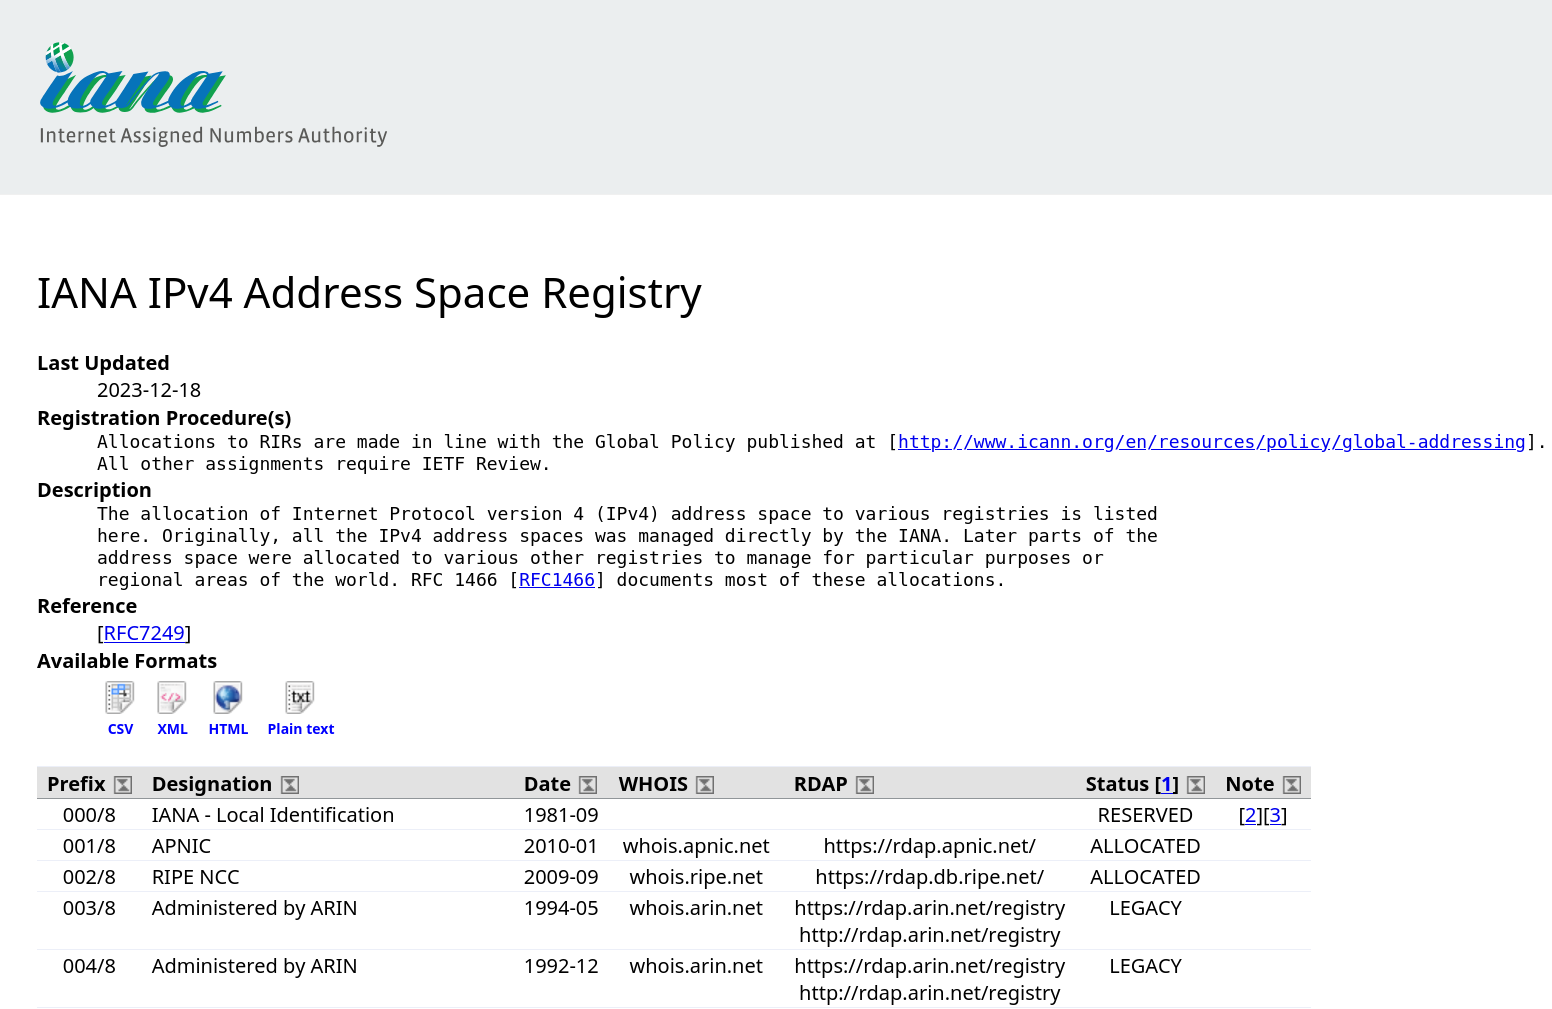
\includegraphics[width=\textwidth]{../arp/iana-registry-screenshot}
\end{frame}

\begin{frame}{}
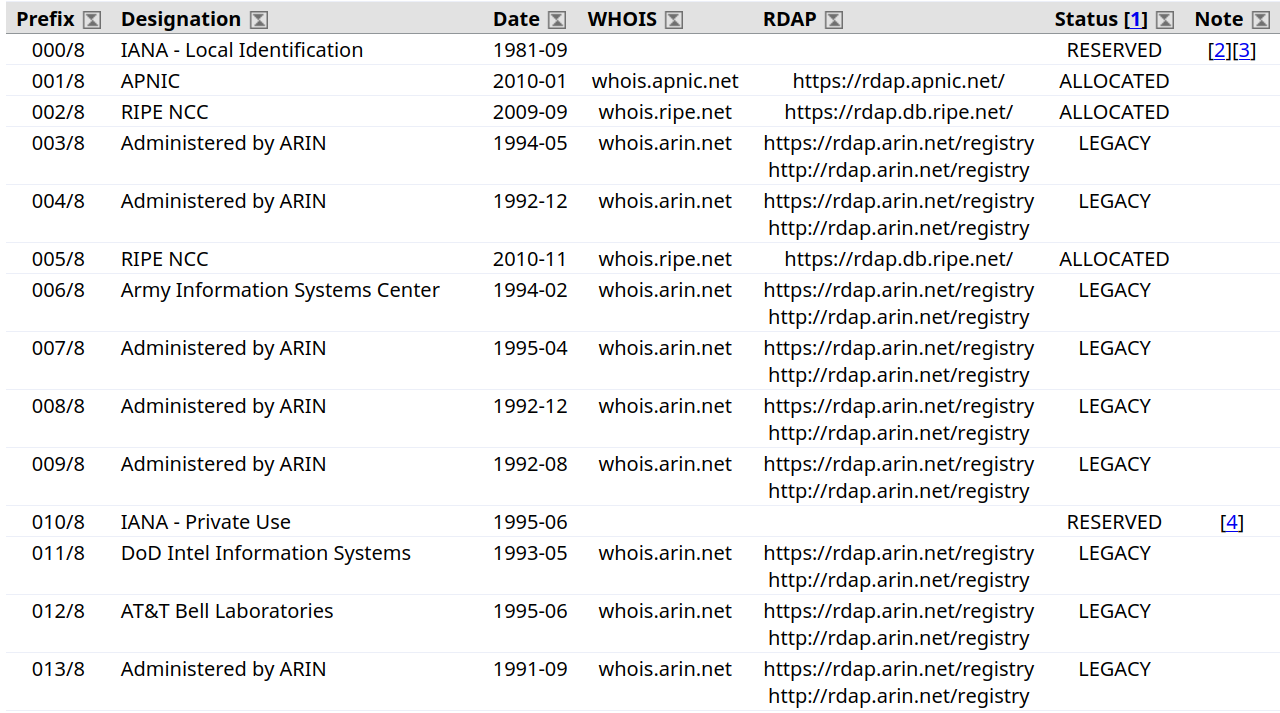
\includegraphics[width=\textwidth]{../arp/iana-ipv4-allocs}
(and 241 more)
\end{frame}

\begin{frame}[fragile]{}
\begin{tikzpicture}
\node (v6 space top) {
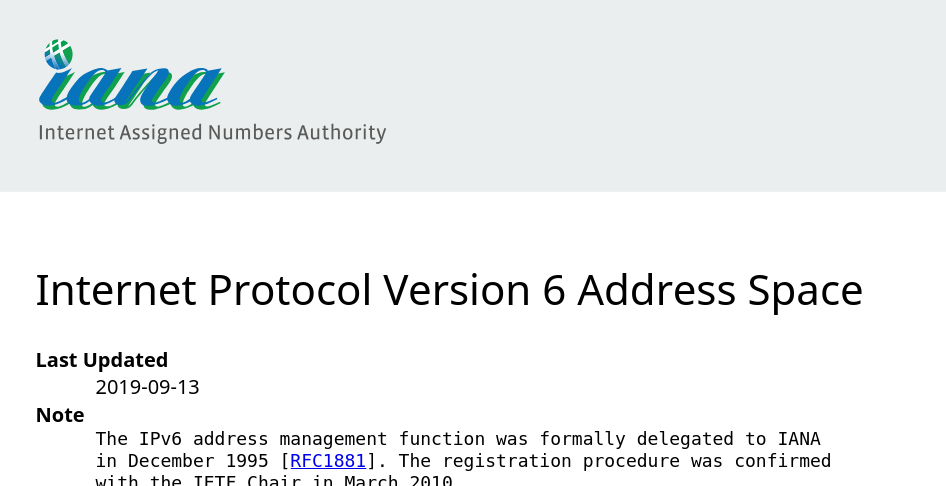
\includegraphics[width=8cm]{../arp/iana-v6-addr-top} 
};
\node[anchor=north,font=\Huge,inner sep=1mm] (v6 space ldots) at ([yshift=-1mm]v6 space top.south) {\ldots};
\node[anchor=north] at (v6 space ldots.north) {
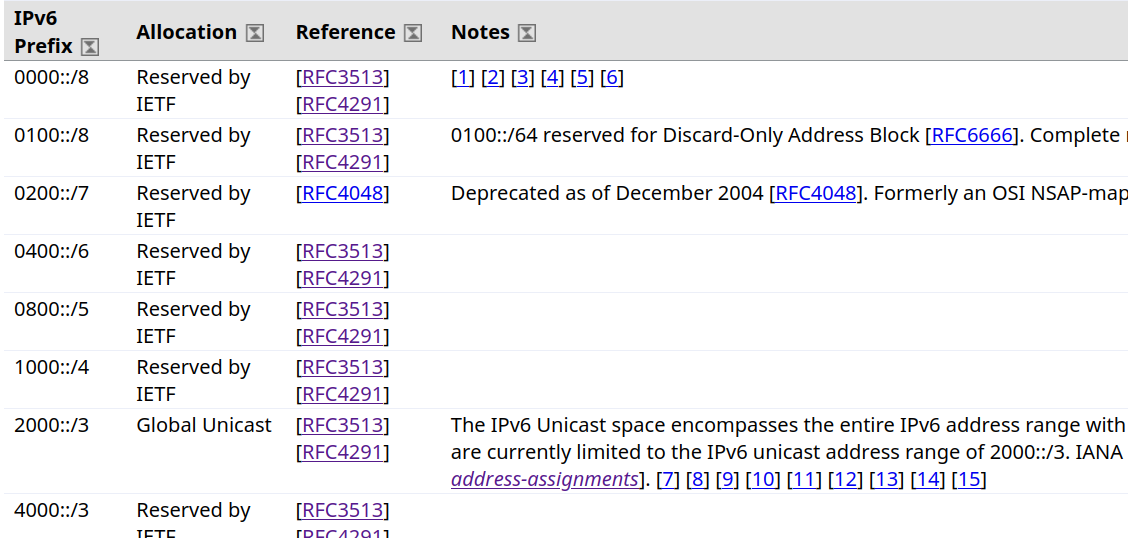
\includegraphics[width=8cm]{../arp/iana-v6-addr-bottom2}
};
\node[anchor=north west] at (v6 space top.north east) {
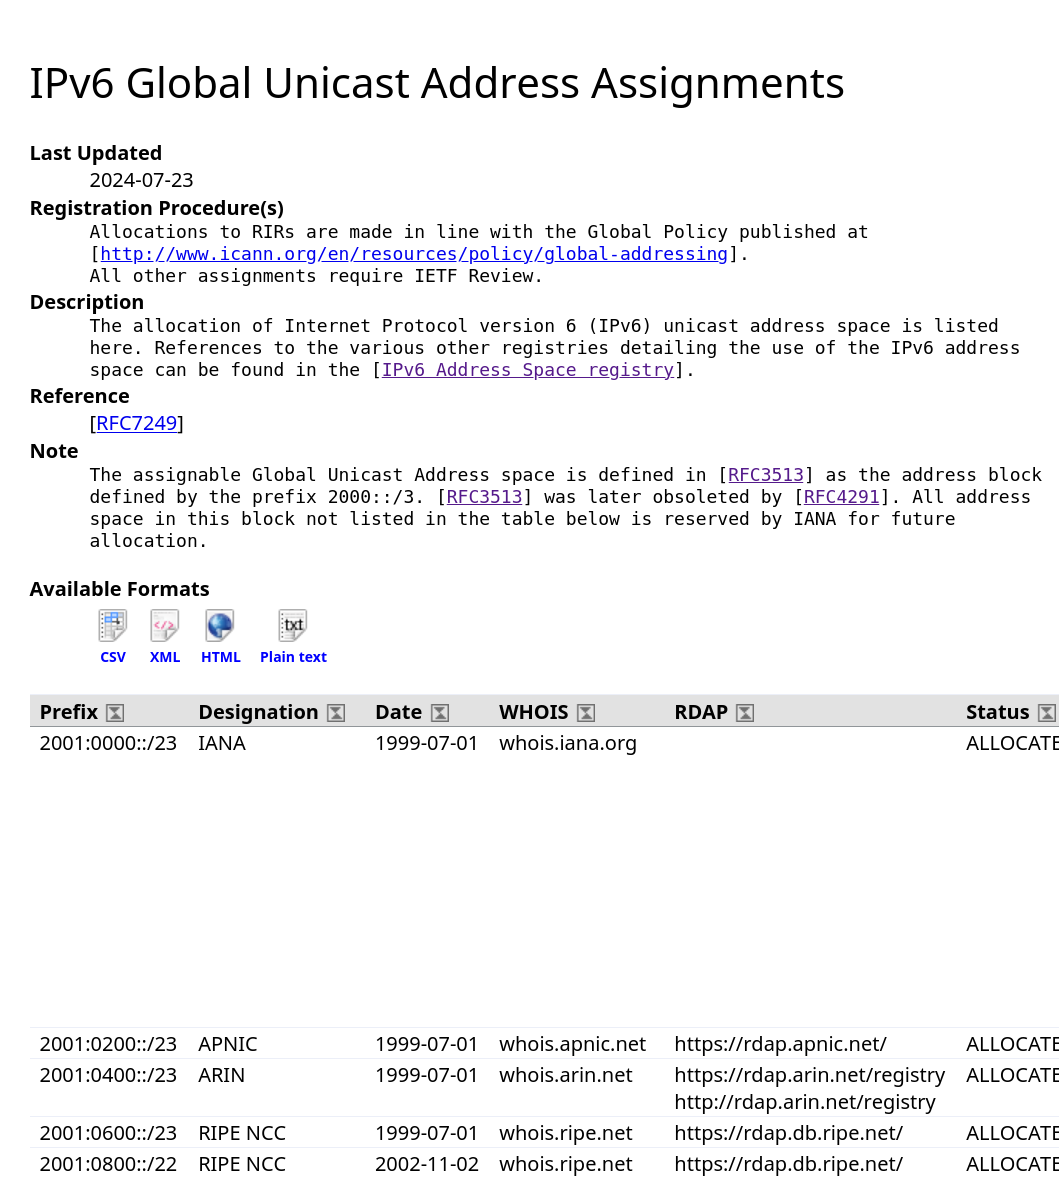
\includegraphics[width=8cm]{../arp/iana-v6-unicast}
};
\end{tikzpicture}
\end{frame}

\begin{frame}{regional internet registries (RIRs)}
\begin{tikzpicture}
\node[inner sep=1mm] (rir) {
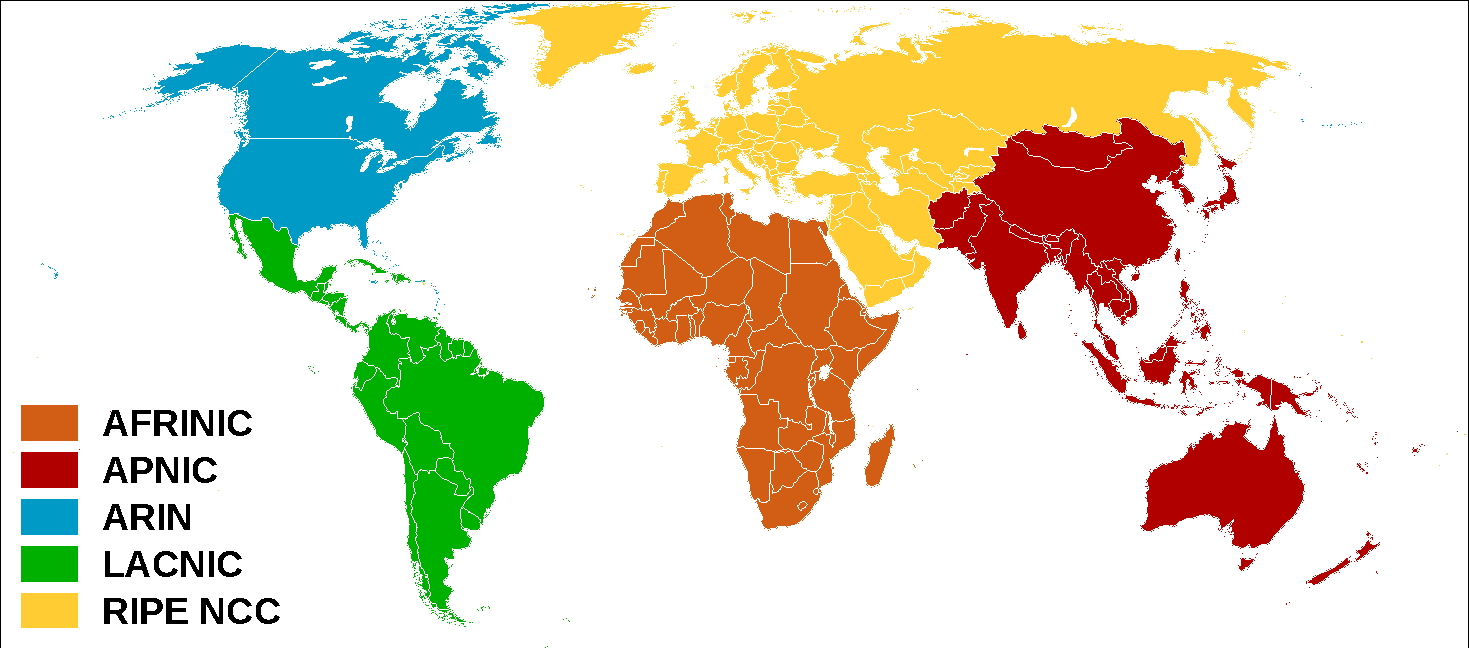
\includegraphics[height=0.35\textheight]{Regional_Internet_Registries_world_map.pdf} 
};
\node[align=left,anchor=north west,font=\scriptsize] at (rir.north east) {
map from Wikimedia Commons, \\
users Dork, Canuckguy et al, S\'emhur, CC-BY-SA 3.0
};
\end{tikzpicture}
\begin{itemize}
\item most useful addresses managed by RIRs
    \begin{itemize}
    \item African Network Information Centre (AFRINIC)
    \item American Registry for Internet Numbers (ARIN)
    \item Asia Pacific Network Information Centre (APNIC)
    \item Latin American and Carribean Network Information Centre (LACNIC)
    \item R\'eseaux IP Europ\'eens Network Coordination Centre (RIPE NCC)
    \end{itemize}
\end{itemize}
\end{frame}

\begin{frame}{RIR suballocations}
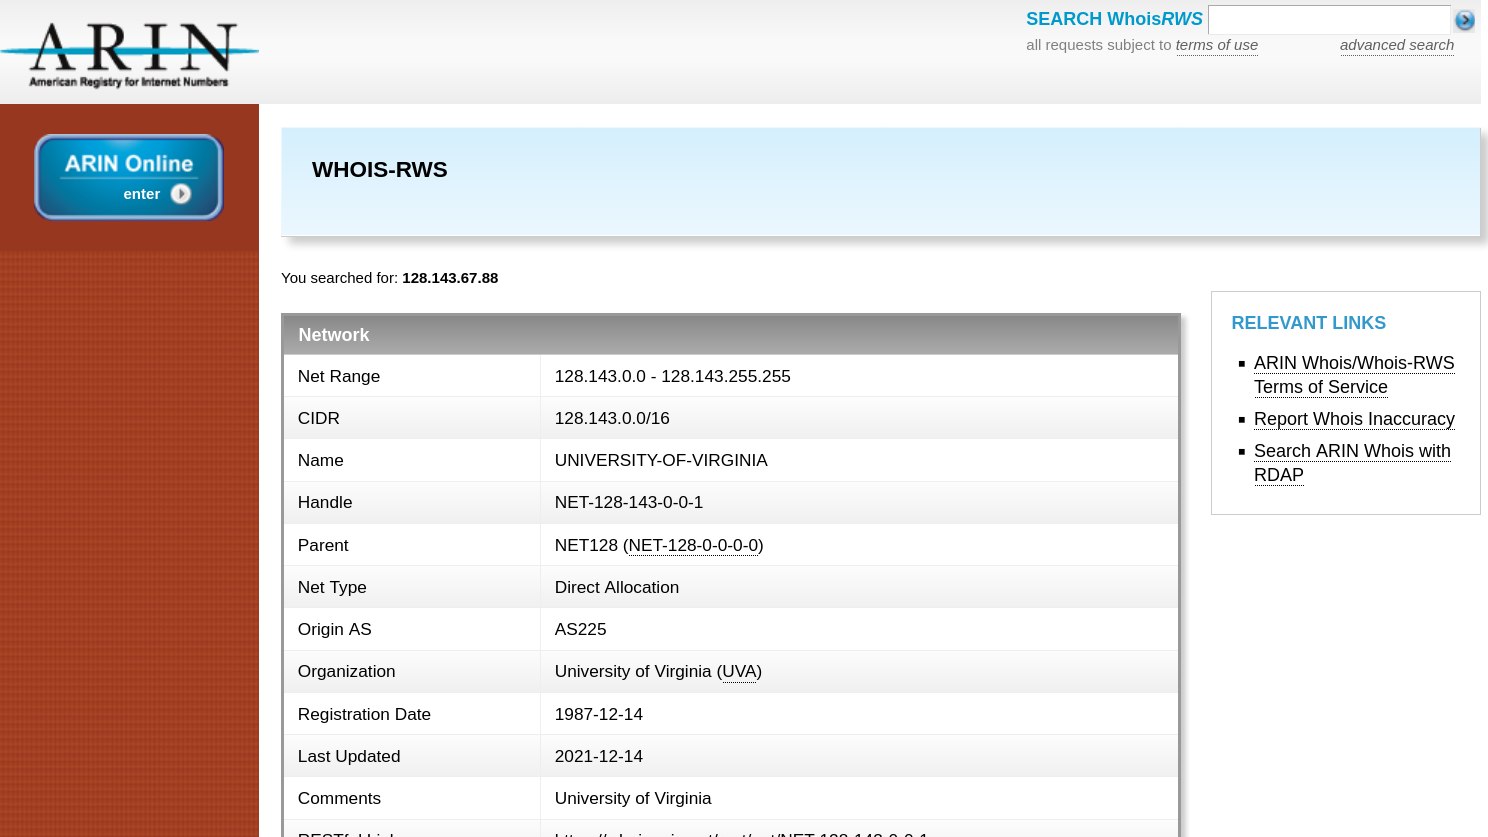
\includegraphics[width=\textwidth]{../arp/arin-whois-virginia}
\end{frame}

\begin{frame}{special IPv4 addresses}
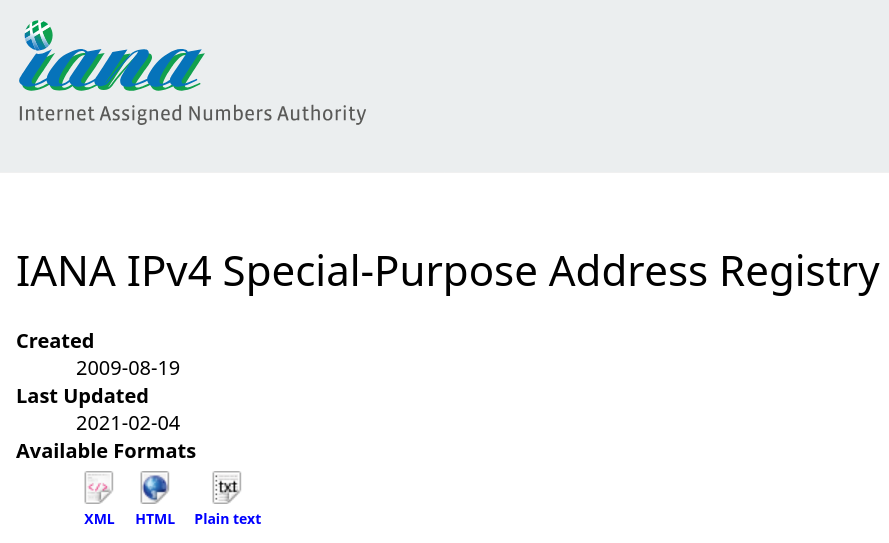
\includegraphics[width=\textwidth]{../arp/iana-special-ipv4-header}
\end{frame}

\begin{frame}{special IPv4 addresses}
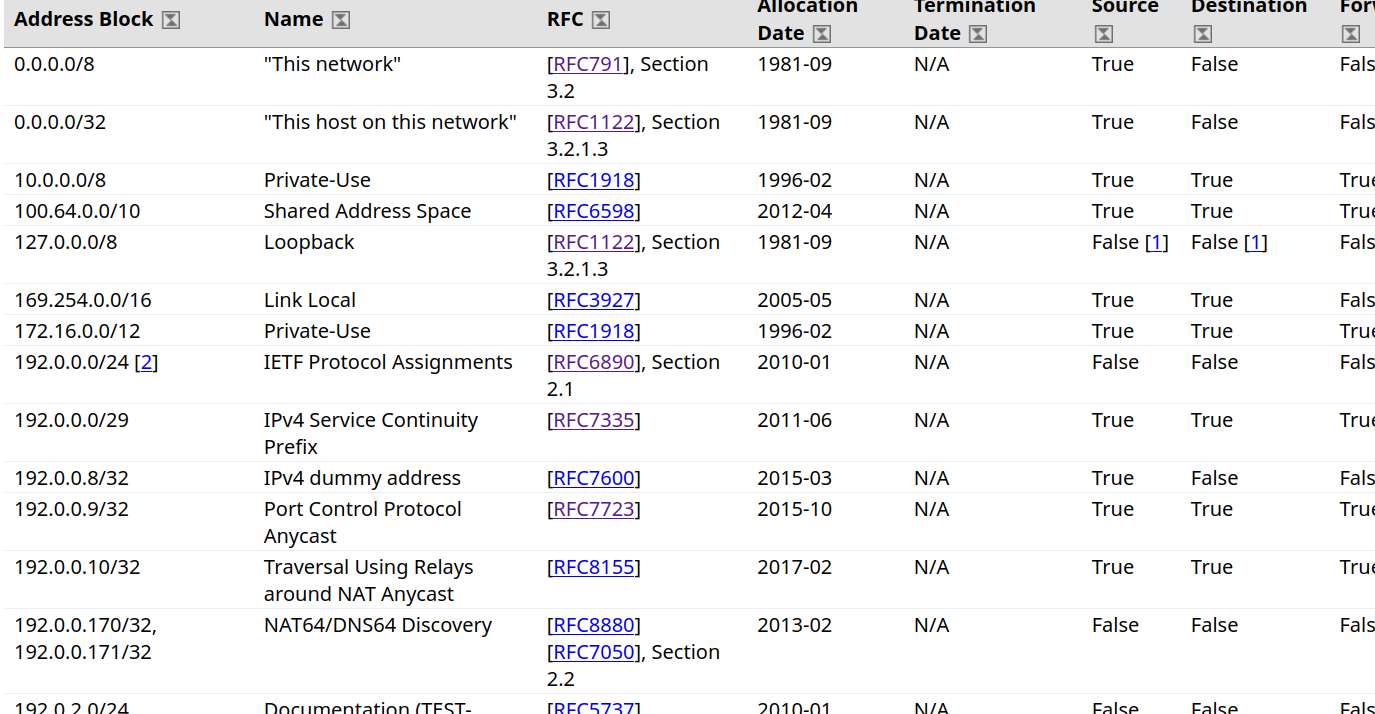
\includegraphics[width=\textwidth]{../arp/iana-special-ipv4-detail}
\end{frame}

\begin{frame}{selected special IP addresses}
\begin{itemize}
\item loopback (current machine) --- {\tt 127/8} (v4), {\tt ::1/128} (v6)
\item link-local (current network only) ---
    \begin{itemize}
    \item {\tt 169.254/16} (v4), {\tt ff80::/10} (v6)
    \end{itemize}
\item private use (non-public networks only) --- \\
    \begin{itemize}
    \item {\tt 192.168/16}, {\tt 172.16/12}, {\tt 10/8} (v4), (kinda) {\tt fc00::/7} (v6)
    \end{itemize}
\item multicast groups and related --- {\tt 224/4} (v4), {\tt ff00::/8} (v6)
    \begin{itemize}
    \item multiple nodes can be part of a single ``multicast group''
    \end{itemize}
\item broadcast (all on current network) --- 
    \begin{itemize}
    \item {\tt 255.255.255.255}, {\tt ff01::1}
    \end{itemize}
\item ``future use'' --- 
    \begin{itemize}
    \item rest of {\tt 240/4} (v4), {\tt 4000::}---{\tt efff::} (v6)
    \end{itemize}
\end{itemize}
\end{frame}


\subsection{which link-local addresses}
\begin{frame}{which link local?}
    \begin{itemize}
    \item ``link local'': \texttt{169.254/16}, \texttt{fe80::/10}
    \item specific to each local network
    \vspace{.5cm}
    \item \texttt{fe80::17} on network A != \texttt{fe80::17} on network B
    \vspace{.5cm}
    \item problem: machine can be connected to two networks
    \item<2-> solution: \texttt{fe80::17\%A} versus \texttt{fe80::17\%B}
    \item<3-> what about IPv4? uh... too bad?
        \begin{itemize}
        \item ``There is no standard or obvious solution to this problem\ldots
        must be done explicitly through other means. The specification does not stipulate
        those means.'' --- RFC 3927, section 3.2
        \end{itemize}
    \end{itemize}
\end{frame}



\section{routing versus switching}
\subsection{tables}
\usetikzlibrary{fit,matrix}
\usetikzlibrary{arrows.meta,calc,shapes}
\providecommand{\computer}{%
    
\includegraphics[width=1cm]{../common/Noun_project_216.pdf}
}
\providecommand{\switch}{%
    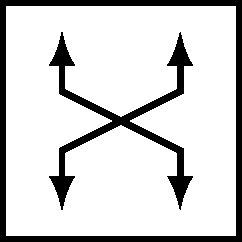
\includegraphics[width=0.9cm]{../common/fig-switch.pdf}
}
\providecommand{\router}{%
    
\includegraphics[width=0.9cm]{../common/fig-router.pdf}
}
\begin{frame}{switch v router: tables}
\begin{tikzpicture}
\matrix[tight matrix,
    nodes={minimum height=.6cm},
    column 1/.style={nodes={text width=5cm,font=\small\tt}},
    column 2/.style={nodes={text width=1cm,font=\small\tt}},
    row 1/.style={nodes={font=\small}},
    label={north:switch (`bridge') table},
] (bridge table) {
MAC address \& port \\
00:11:22:33:44:55 \& 1 \\
00:33:00:01:02:aa \& 2 \\
00:44:00:01:02:bb \& 3 \\
\ldots \& \ldots \\
\normalfont default \& (all) \\
};
\matrix[tight matrix,
    nodes={minimum height=.6cm},
    column 1/.style={nodes={text width=4.5cm,font=\small\tt}},
    column 2/.style={nodes={text width=2cm,font=\small\tt,alt=<4>{fill=red!10}}},
    column 3/.style={nodes={text width=1cm,font=\small\tt,alt=<3>{fill=red!10}}},
    row 1/.style={nodes={font=\small}},
    label={north:routing table},
    anchor=north west
] (route table) at ([xshift=.5cm]bridge table.north east){
IP addresses \& gateway \& iface \\
2001:0db8:40::/48 \& --- \& int \\
3fff:1000:19::/48 \& --- \& ext \\
\ldots \& \ldots \& \ldots \\
\normalfont default \& fe80::17 \& ext \\
};
\begin{visibleenv}<2>
\node[
    draw=red,ultra thick,fit=(bridge table),
] (bridge table around) {};
\node[align=left,anchor=north west] at (bridge table around.south west) {
    one logical device with multiple ports \\
    not in table: always broadcast
};
\end{visibleenv}
\begin{visibleenv}<3->
\node[
    draw=red,ultra thick,fit=(route table),
] (route table around) {};
\end{visibleenv}
\begin{visibleenv}<3>
\node[align=left,anchor=north] at (route table around.south) {
    `interface' = which network \\
    ~ \\
    one interface might have multiple ports \\
    that are `bridged' together \\
};
\end{visibleenv}
\begin{visibleenv}<4>
\node[align=left,anchor=north] at (route table around.south) {
    gateway = who to send to next \\
    no gateway = `direct' to destination \\
    ~ \\
    need to have specific destination \\
    to send to on interface
};
\end{visibleenv}
\end{tikzpicture}
\end{frame}

\begin{frame}{trivial tables}
\begin{itemize}
\item let's say we're connected to ONE interface with ONE port
\item<2-> tables are really trivial:
\end{itemize}
\begin{visibleenv}<2->
\begin{tikzpicture}
\matrix[tight matrix,
    nodes={minimum height=.6cm},
    column 1/.style={nodes={text width=2.5cm,font=\small}},
    column 2/.style={nodes={text width=1.5cm,font=\small}},
    row 1/.style={nodes={font=\small}},
    label={north:switch (`bridge') table},
] (bridge table) {
MAC address \& port \\
default \& the port \\
};
\matrix[tight matrix,
    nodes={minimum height=.6cm},
    column 1/.style={nodes={text width=4.5cm,font=\small\tt}},
    column 2/.style={nodes={text width=2.5cm,font=\small\tt,alt=<4>{fill=red!10}}},
    column 3/.style={nodes={text width=2.5cm,font=\fontsize{9}{10}\tt,alt=<3>{fill=red!10}}},
    row 1/.style={nodes={font=\small}},
    label={north:routing table (IPv6)},
    anchor=north west
] (route table) at ([xshift=.5cm]bridge table.north east){
IP addresses \& gateway \& iface \\
2001:0db8:40::/48 \& --- \& the interface \\
\normalfont default \& fe80::17 \& the interface \\
};
\matrix[tight matrix,
    nodes={minimum height=.6cm},
    column 1/.style={nodes={text width=4.5cm,font=\small\tt}},
    column 2/.style={nodes={text width=2.5cm,font=\small\tt,alt=<4>{fill=red!10}}},
    column 3/.style={nodes={text width=2.5cm,font=\fontsize{9}{10}\tt,alt=<3>{fill=red!10}}},
    row 1/.style={nodes={font=\small}},
    label={north:routing table (IPv4)},
    anchor=north west,
] (route table v4) at ([yshift=-.8cm]route table.south west){
IP addresses \& gateway \& iface \\
192.0.2.0/24 \& --- \& the interface \\
\normalfont default \& 192.0.2.1 \& the interface \\
};
\end{tikzpicture}
\end{visibleenv}
\end{frame}

\subsection{tables}
\usetikzlibrary{fit,matrix}
\usetikzlibrary{arrows.meta,calc,shapes}
\providecommand{\computer}{%
    
\includegraphics[width=1cm]{../common/Noun_project_216.pdf}
}
\providecommand{\switch}{%
    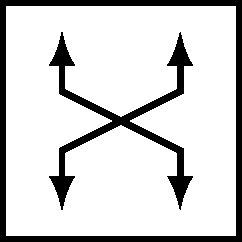
\includegraphics[width=0.9cm]{../common/fig-switch.pdf}
}
\providecommand{\router}{%
    
\includegraphics[width=0.9cm]{../common/fig-router.pdf}
}

\begin{frame}{switch v router: on the wires}
\begin{tikzpicture}
\tikzset{
    computer/.style={inner sep=0mm,outer sep=0mm,execute at begin node={\computer}},
    switch/.style={inner sep=0mm,outer sep=0mm,execute at begin node={\switch}},
    router/.style={inner sep=-1mm,outer sep=0mm,execute at begin node={\router},circle},
    connect/.style={draw,very thick,Latex-Latex},
    connect big/.style={draw,ultra thick,Latex-Latex},
    addr label/.style={align=left,font=\fontsize{9}{10}\selectfont\tt},
}
\node[computer,label={[addr label]south:MAC 00:\ldots:AA\\IP 10.0.1.2},alt=<5>{draw=red,ultra thick,fill=red!10}] (n1-c1) at (0, -2.5) {};
\node[computer,label={[addr label]south:MAC 04:\ldots:BB\\IP 10.0.1.3}]  (n1-c2) at (0, 0) {};
\node[switch] (n1-s1) at (3,-1) {};
\node[switch] (n1-s2) at (5,-4) {};
\node[computer,label={[addr label]south:MAC 05:\ldots:CC\\IP 10.0.1.4}] (n1-c3) at (1, -5) {};
\draw[connect] (n1-c1) -- (n1-s1);
\draw[connect] (n1-c2) -- (n1-s1);
\draw[connect] (n1-c3) -- (n1-s2);
\draw[connect big] (n1-s1) -- (n1-s2);
\node[router,label={[addr label]south:MAC \myemph<5-6>{02:\ldots:DD} / 02:\ldots:DE\\IP: 10.0.1.1 / 10.0.2.15},alt=<5-6>{fill=red!10,draw=red,ultra thick}] (n1n2) at (9, -5) {};
\node[switch] (n2-s1) at (11, -3) {};
\node[computer,label={[addr label]south:MAC 03:\ldots:EE\\IP: \myemph<5>{10.0.2.2}},alt=<5>{draw=red,ultra thick,fill=red!10}] (n2-c1) at (12.5, -4) {};
\draw[connect](n2-s1) -- (n2-c1);

\draw[connect big] (n1-s2) -- (n1n2);
\draw[connect big] (n2-s1) -- (n1n2);
\begin{pgfonlayer}{bg}
    \begin{visibleenv}<2->
        \path[overlay,draw=violet,fill=violet!10]
            (-1.3, -7) -- (5, -7) -- (9, -7) -- (9, -3) -- (4, .75) -- (-1.3, .75) -- cycle;
        \path[overlay,draw=green,fill=green!10]
            (7, 0) -- (8, -2) -- (9, -3) -- (9, -7) -- (13.5, -7) -- (13.5, 0) -- cycle;
        \node[anchor=south,font=\tt] at (5, -7) {10.0.1.0/24};
        \node[anchor=south,font=\tt] at (11, -7) {10.0.2.0/24};
    \end{visibleenv}
\end{pgfonlayer}
\begin{visibleenv}<3->
        \foreach \x [remember=\x as \lastx (initially n1-c1)] in {n1-s1,n1-s2,n1n2,n2-s1,n2-c1} {
            \path[draw,dotted,blue,line width=1mm,arrows=-Latex] (\lastx) -- (\x);
        }
\end{visibleenv}
\begin{visibleenv}<4->
    \path[draw,blue,thick] ($(n1-c1)!0.5!(n1-s1)$) -- (3.7, -1) ++ (0, 1.) coordinate (n1 frame base);
    \node[font=\fontsize{9}{10}\tt,anchor=north west] (n1 outer) at (n1 frame base) {
        00:\ldots:AA\hspace{1mm}$\rightarrow$\myemph<5>{\hspace{1mm}02:\ldots:DD}
    };
    \node[align=left,font=\fontsize{9}{10}\tt,anchor=north west,draw=black!50,very thick,
          alt=<6>{fill=red!10},
    ] (n1 inner) at ([xshift=1mm]n1 outer.south west) {
        10.0.1.3 $\rightarrow$ \myemph<5>{10.0.2.2} \\
        (actual data)
    };
    \path (12, -0) ++ (-2.25, 0.5) coordinate (n2 frame base);
    \node[font=\fontsize{9}{10}\tt,anchor=north west] (n2 outer) at (n2 frame base) {
        02:\ldots:DE\hspace{1mm}$\rightarrow$\hspace{1mm}03:\ldots:EE
    };
    \node[align=left,font=\fontsize{9}{10}\tt,anchor=north west,draw=black!50,very thick,
          alt=<6>{fill=red!10}
    ] (n2 inner) at ([xshift=1mm]n2 outer.south west) {
        10.0.1.3 $\rightarrow$ 10.0.2.2 \\
        (actual data)
    };
\end{visibleenv}
\begin{pgfonlayer}{bg}
    \begin{visibleenv}<4->
    \node[inner sep=0mm,fill=white,draw=blue,very thick,
          fit={(n1 outer) (n1 inner) ([yshift=-1mm]n1 inner.south) ([xshift=1mm]n1 inner.east)}
    ] (n1 box) {};
    \path[draw,blue,thick] ($(n1-s1)!0.5!(n1-s2)$) -- (n1 box);
    \path[draw,blue,thick] ($(n1-s2)!0.5!(n1n2)$) -- (n1 box);
    \node[inner sep=0mm,fill=white,draw=blue,very thick,
          fit={(n2 outer) (n2 inner) ([yshift=-1mm]n2 inner.south) ([xshift=1mm]n2 inner.east)}
    ] (n2 box) {};
    \path[draw,blue,thick] ($(n2-s1)!0.5!(n1n2)$) -- ([xshift=.5cm]n2 box.south west);
    \path[draw,blue,thick] ($(n2-c1)!0.5!(n2-s1)$) -- ([xshift=2cm]n2 box.south west);
    \end{visibleenv}
\end{pgfonlayer}
\begin{visibleenv}<5>
    \node[fill=white,draw=red,ultra thick,align=left] at (3, -5) {
        MAC address = on \textit{local} network \\
        IP address = somewhere else
    };
\end{visibleenv}
\begin{visibleenv}<7>
    \draw[red, ultra thick] (n1 inner) -- (n2 inner)
        node[inner sep=0mm,
             midway,pin={[pin edge={red,ultra thick},fill=white,draw=red,thick,align=center]-90:IP packet copied as is\\placed in new frame}] {};
\end{visibleenv}
% FIXME:    show packets involved
% FIXME:    show frames involved
% FIXME:    show bridge/routing table
\end{tikzpicture}
\end{frame}

\begin{frame}{steps at the sender}
\begin{tikzpicture}
\tikzset{
    computer/.style={inner sep=0mm,outer sep=0mm,execute at begin node={\computer}},
    switch/.style={inner sep=0mm,outer sep=0mm,execute at begin node={\switch}},
    router/.style={inner sep=-1mm,outer sep=0mm,execute at begin node={\router},circle},
    connect/.style={draw,very thick,Latex-Latex},
    connect big/.style={draw,ultra thick,Latex-Latex},
    addr label/.style={align=left,font=\fontsize{9}{10}\selectfont\tt},
}
\node[computer,label={[addr label]south:MAC 00:\ldots:AA\\IP 10.0.1.2},alt=<2->{draw=red,ultra thick,fill=red!10}] (n1-c1) at (0, -2.5) {};
\node[font=\bfseries] at (n1-c1) {src};
\node[computer,label={[addr label]south:MAC 04:\ldots:BB\\IP 10.0.1.3}]  (n1-c2) at (0, 0) {};
\node[switch] (n1-s1) at (3,-1) {};
\node[switch] (n1-s2) at (5,-4) {};
\node[computer,label={[addr label]south:MAC 05:\ldots:CC\\IP 10.0.1.4}] (n1-c3) at (1, -5) {};
\draw[connect] (n1-c1) -- (n1-s1);
\draw[connect] (n1-c2) -- (n1-s1);
\draw[connect] (n1-c3) -- (n1-s2);
\node[router,label={[addr label]south:MAC 02:\ldots:DD / 02:\ldots:DE\\IP: 10.0.1.1 / 10.0.2.15}] (n1n2) at (9, -5) {};
\draw[connect big] (n1-s1) -- (n1-s2);
\draw[connect big] (n1-s2) -- (n1n2);
    \foreach \x [remember=\x as \lastx (initially n1-c1)] in {n1-s1,n1-s2,n1n2} {
        \path[draw,dotted,blue,line width=1mm,arrows=-Latex] (\lastx) -- (\x);
    }

    \path (3.7, -1) ++ (0, 1.) coordinate (n1 frame base);
    \begin{visibleenv}<3>
        \node[font=\fontsize{9}{10}\tt,anchor=north west] (n1 outer pre 1) at (n1 frame base) {
            \myemph<4>{00:\ldots:AA}\hspace{1mm}$\rightarrow$\hspace{1mm}???????
        };
    \end{visibleenv}
    \begin{visibleenv}<4>
        \node[font=\fontsize{9}{10}\tt,anchor=north west] (n1 outer pre 2) at (n1 frame base) {
            \myemph<4>{00:\ldots:AA}\hspace{1mm}$\rightarrow$\hspace{1mm}\myemph<4>{\normalfont 10.0.1.1's MAC}
        };
    \end{visibleenv}
    \begin{visibleenv}<5->
        \node[font=\fontsize{9}{10}\tt,anchor=north west] (n1 outer) at (n1 frame base) {
            00:\ldots:AA\hspace{1mm}$\rightarrow$\hspace{1mm}02:\ldots:DD
        };
    \end{visibleenv}
   \begin{visibleenv}<2->
        \node[
            align=left,font=\fontsize{9}{10}\tt,anchor=north west,draw=black!50,very thick,
            alt=<2>{fill=red!10},
        ] (n1 inner) at ([xshift=1mm]n1 outer.south west) {
            10.0.1.2 $\rightarrow$ \myemph<5>{10.0.2.2}\\
            (actual data)
        };
    \end{visibleenv}
    \begin{visibleenv}<2>
        \path[draw=red,ultra thick,arrows=Latex-](n1 inner.east) -- ++(1cm, 0cm) node[right] {
            packet from upper layer
        };
    \end{visibleenv}
    \begin{visibleenv}<3>
        \path[draw=red,ultra thick,arrows=Latex-,align=left] (n1 outer pre 1.east) -- ++(1cm, 0cm) node[right] {
            need to send at link layer
        };
    \end{visibleenv}
    \begin{visibleenv}<4>
        \path[draw=red,ultra thick,arrows=Latex-,align=left] (n1 outer pre 2.east) -- ++(1cm, 0cm) node[right] {
            routing table says: \\
            to 10.0.1.1 \\
            but need MAC address
        };
    \end{visibleenv}
    \begin{visibleenv}<5>
        \path[draw=red,ultra thick,arrows=Latex-,align=left] (n1 outer pre 1.east) -- ++(1cm, 0cm) node[right] {
            need IP:MAC address table \\
            called neighbor table \\
            or ARP table
        };
    \end{visibleenv}
\begin{pgfonlayer}{bg}
    \begin{visibleenv}<3->
    \node[inner sep=0mm,fill=white,draw=blue,very thick,
          fit={(n1 outer) (n1 inner) ([yshift=-1mm]n1 inner.south) ([xshift=1mm]n1 inner.east)}
    ] (n1 box) {};
    \end{visibleenv}
\end{pgfonlayer}
\tikzset{
    route table/.style={
        matrix of nodes,ampersand replacement=\&,
        nodes={execute at begin node={\strut}},
        column 1/.style={nodes={draw,thin,text width=3cm,font=\fontsize{8}{9}\tt,minimum height=0.4cm,inner sep=.1mm}},
        column 2/.style={nodes={draw,thin,text width=2cm,font=\fontsize{8}{9}\tt,minimum height=0.4cm,inner sep=.1mm}},
        column 3/.style={nodes={draw,thin,text width=1cm,font=\fontsize{8}{9}\tt,minimum height=0.4cm,inner sep=.1mm}},
        row 1/.style={nodes={draw=none,font=\fontsize{8}{9}\selectfont}},
    }
}
%% FIXME: show this with build of IP packet without extra stuff
\begin{pgfonlayer}{fg}
    \begin{visibleenv}<4-5>
    \matrix[
        route table,anchor=north west,
        label={[label distance=0mm,font=\small,alias=route table label]north:src's routing table},
        inner sep=0mm,
        row 3/.style={alt=<4>{nodes={draw=red,fill=red!10}}},
    ] (route table) at (7, -2){
    address \& gateway \& iface \\
    10.0.1.0/24 \& --- \& wired \\
    default \& |[alt=<5>{fill=red!10}]| 10.0.1.1 \& wired \\
    };
    \end{visibleenv}
    \begin{visibleenv}<5->
    \matrix[
        route table,anchor=north west,
        label={[label distance=0mm,font=\small,alias=arp table label]north:src's neighbor table},
        column 1/.style={nodes={draw,thin,text width=2cm,font=\fontsize{8}{9}\tt,minimum height=0.4cm,inner sep=.1mm}},
        column 2/.style={nodes={draw,thin,text width=2cm,font=\fontsize{8}{9}\tt,minimum height=0.4cm,inner sep=.1mm}},
        column 3/.style={nodes={draw,thin,text width=1cm,font=\fontsize{8}{9}\tt,minimum height=0.4cm,inner sep=.1mm}},
        row 3/.style={alt=<4>{nodes={draw=red,fill=red!10}}},
    ] (arp table) at ([yshift=-1cm]route table.south west){
    IP address \& MAC addresss \\
    |[alt=<5>{fill=red!10}]| 10.0.1.1 \& |[alt=<5>{fill=red!10}]| 05:\ldots:DD \\
    10.0.1.4 \& 05:\ldots:CC \\
    };
    \end{visibleenv}
\end{pgfonlayer}
\begin{visibleenv}<4-5>
    \node[fill=white,draw,thick,alt=<4>{ultra thick,draw=red},fit=(route table) (route table label),inner sep=.5mm] {};
\end{visibleenv}
\begin{visibleenv}<5>
    \node[fill=white,draw,thick,alt=<5>{ultra thick,draw=red},fit=(arp table) (arp table label),inner sep=1mm] {};
\end{visibleenv}
% FIXME: show what happens on router
\end{tikzpicture}
\end{frame}

\begin{frame}{steps at the router}
\begin{tikzpicture}
\tikzset{
    computer/.style={inner sep=0mm,outer sep=0mm,execute at begin node={\computer}},
    switch/.style={inner sep=0mm,outer sep=0mm,execute at begin node={\switch}},
    router/.style={inner sep=-1mm,outer sep=0mm,execute at begin node={\router},circle},
    connect/.style={draw,very thick,Latex-Latex},
    connect partial/.style={draw=black!25,overlay},
    connect big/.style={draw,ultra thick,Latex-Latex},
    addr label/.style={align=left,font=\fontsize{9}{10}\selectfont\tt},
}
%\node[computer,label={[addr label]south:MAC 00:\ldots:AA\\IP 10.0.1.2}] (n1-c1) at (0, -2.5) {};
%\node[computer,label={[addr label]south:MAC 04:\ldots:BB\\IP 10.0.1.3}]  (n1-c2) at (0, 0) {};
%\node[switch] (n1-s1) at (3,-1) {};
\node[overlay] (n1-s1) at (3,-1) {};
\node[switch] (n1-s2) at (5,-4) {};
%\node[computer,label={[addr label]south:MAC 05:\ldots:CC\\IP 10.0.1.4}] (n1-c3) at (1, -5) {};
\node[overlay] (n1-c3) at (1, -5) {};
%\draw[connect] (n1-c1) -- (n1-s1);
%\draw[connect] (n1-c2) -- (n1-s1);
\draw[connect,connect partial] (n1-c3) -- (n1-s2);
\draw[connect big,connect partial, ] (n1-s1) -- (n1-s2);
\node[router,label={[addr label]south:MAC {02:\ldots:DD} / 02:\ldots:DE\\IP: 10.0.1.1 / 10.0.2.15}] (n1n2) at (9, -5) {};
\node[font=\bfseries,red] at (n1n2) {rtr}; 
\node[switch] (n2-s1) at (11, -3) {};
%\node[computer,label={[addr label]south:MAC 03:\ldots:EE\\IP: {10.0.2.2}}] (n2-c1) at (12.5, -4) {};
\node[overlay] (n2-c1) at (12.5, -4) {};
\draw[connect,connect partial](n2-s1) -- (n2-c1);

\draw[connect big] (n1-s2) -- (n1n2);
\draw[connect big] (n2-s1) -- (n1n2);
\begin{pgfonlayer}{bg}
    \begin{scope}[overlay]
        \path[overlay,draw=violet,fill=violet!10]
            (-1.3, -7) -- (5, -7) -- (9, -7) -- (9, -3) -- (4, .75) -- (-1.3, .75) -- cycle;
        \path[overlay,draw=green,fill=green!10]
            (7, 0) -- (8, -2) -- (9, -3) -- (9, -7) -- (13.5, -7) -- (13.5, 0) -- cycle;
        \node[anchor=south,font=\tt] at (5, -7) {10.0.1.0/24};
        \node[anchor=south,font=\tt] at (11, -7) {10.0.2.0/24};
    \end{scope}
\end{pgfonlayer}
%        \foreach \x [remember=\x as \lastx (initially n1-s2)] in {n1-s1,n1-s2,n1n2,n2-s1,n2-c1} {
%            \path[draw,dotted,blue,line width=1mm,arrows=-Latex] (\lastx) -- (\x);
%        }
%    \path[draw,blue,thick] ($(n1-c1)!0.5!(n1-s1)$) -- (3.7, -1) ++ (0, 1.) coordinate (n1 frame base);
    \node[font=\fontsize{9}{10}\tt,anchor=north west] (n1 outer) at (n1 frame base) {
        00:\ldots:AA\hspace{1mm}$\rightarrow${\hspace{1mm}02:\ldots:DD}
    };
    \node[align=left,font=\fontsize{9}{10}\tt,anchor=north west,draw=black!50,very thick,
    ] (n1 inner) at ([xshift=1mm]n1 outer.south west) {
        10.0.1.3 $\rightarrow$ \myemph<2>{10.0.2.2} \\
        (actual data)
    };
    \path (12, -0) ++ (-2.25, 0.5) coordinate (n2 frame base);
\tikzset{
    route table/.style={
        matrix of nodes,ampersand replacement=\&,
        nodes={execute at begin node={\strut}},
        column 1/.style={nodes={draw,thin,text width=3cm,font=\fontsize{8}{9}\tt,minimum height=0.4cm,inner sep=.1mm}},
        column 2/.style={nodes={draw,thin,text width=2cm,font=\fontsize{8}{9}\tt,minimum height=0.4cm,inner sep=.1mm}},
        column 3/.style={nodes={draw,thin,text width=1cm,font=\fontsize{8}{9}\tt,minimum height=0.4cm,inner sep=.1mm}},
        row 1/.style={nodes={draw=none,font=\fontsize{8}{9}\selectfont}},
    }
}
    % route and ARP tables
    \begin{pgfonlayer}{fg}
        \begin{visibleenv}<2->
        \matrix[
            fill=white,
            route table,anchor=north west,
            label={[label distance=0mm,font=\small,alias=route table label]north:rtr's routing table},
            inner sep=0mm,
            row 3/.style={alt=<2>{fill=red!10}},
        ] (route table) at (12, -2){
        address \& gateway \& iface \\
        10.0.1.0/24 \& --- \& left \\
        10.0.2.0/24 \& --- \& right \\
        };
        \end{visibleenv}
        \begin{visibleenv}<4->
        \matrix[
            route table,anchor=north,
            label={[label distance=0mm,font=\small,alias=arp table label]north:rtr's neighbor table for right},
            column 1/.style={nodes={draw,thin,text width=2cm,font=\fontsize{8}{9}\tt,minimum height=0.4cm,inner sep=.1mm}},
            column 2/.style={nodes={draw,thin,text width=2cm,font=\fontsize{8}{9}\tt,minimum height=0.4cm,inner sep=.1mm}},
            column 3/.style={nodes={draw,thin,text width=1cm,font=\fontsize{8}{9}\tt,minimum height=0.4cm,inner sep=.1mm}},
            row 3/.style={alt=<4>{nodes={draw=red,fill=red!10}}},
            fill=white,
            inner sep=0mm,
        ] (arp table) at ([yshift=-1cm]route table.south){
        IP address \& MAC addresss \\
        10.0.2.2 \& 03:\ldots:EE \\
        };
        \end{visibleenv}
    \end{pgfonlayer}

    % out going packet
    \begin{visibleenv}<5->
    \node[font=\fontsize{9}{10}\tt,anchor=north west] (n2 outer) at (n2 frame base) {
        02:\ldots:DE\hspace{1mm}$\rightarrow$\hspace{1mm}03:\ldots:EE
    };
    \node[align=left,font=\fontsize{9}{10}\tt,anchor=north west,draw=black!50,very thick,
    ] (n2 inner) at ([xshift=1mm]n2 outer.south west) {
        10.0.1.3 $\rightarrow$ 10.0.2.2 \\
        (actual data)
    };
    \end{visibleenv}
\begin{pgfonlayer}{bg}
    \node[inner sep=0mm,fill=white,draw=blue,very thick,
          fit={(n1 outer) (n1 inner) ([yshift=-1mm]n1 inner.south) ([xshift=1mm]n1 inner.east)}
    ] (n1 box) {};
    %\path[draw,blue,thick] ($(n1-s1)!0.5!(n1-s2)$) -- (n1 box);
    \path[draw,blue,thick] ($(n1-s2)!0.5!(n1n2)$) -- (n1 box);
    \begin{visibleenv}<5->
    \node[inner sep=0mm,fill=white,draw=blue,very thick,
          fit={(n2 outer) (n2 inner) ([yshift=-1mm]n2 inner.south) ([xshift=1mm]n2 inner.east)}
    ] (n2 box) {};
    \path[draw,blue,thick] ($(n2-s1)!0.5!(n1n2)$) -- ([xshift=.5cm]n2 box.south west);
    %\path[draw,blue,thick] ($(n2-c1)!0.5!(n2-s1)$) -- ([xshift=2cm]n2 box.south west);
    \end{visibleenv}
\end{pgfonlayer}
\end{tikzpicture}
\end{frame}




\section{ARP}

\subsection{neighbor table, filling by hand}
\begin{frame}{making neighbor tables}
    \begin{itemize}
    \item need neighbor table to use IP addresses on network
    \vspace{.5cm}
    \item some options:
        \begin{itemize}
        \item system administrator manually configures
        \item discover dynamically
        \end{itemize}
    \end{itemize}
\end{frame}

\begin{frame}{manual neighbor tables}
\begin{itemize}
\item on Linux, can run some commands
\vspace{.5cm}
\item {\tt ip niegh add 10.0.2.2 dev right \\ \hspace{3cm}lladdr 03:05:\ldots:EE permanent}
    \begin{itemize}
    \item (newer interface, also supports IPv6)
    \end{itemize}
\item {\tt arp -i right -s 10.0.2.2 03:05:\ldots:EE}
    \begin{itemize}
    \item IPv4 only; does not allow setting validity duration
    \end{itemize}
\end{itemize}
\end{frame}


\subsection{ARP, ND}

\usetikzlibrary{arrows.meta,calc,fit,matrix,shapes}
\begin{frame}{ARP/ND protocols}
    \begin{itemize}
    \item filling in tables dynamically?
    \item key idea: ask \textit{everyone} on network
    \item entity with that IP address responds
    \vspace{.5cm}
    \item IPv4: Address Resolution Protocol (ARP)
    \item IPv6: ICMPv6 Neighbor Discovery (ND)
        \begin{itemize}
        \item ICMP = Internet Control Message Protocol
        \end{itemize}
    \end{itemize}
\end{frame}

\begin{frame}{ARP messages}
\begin{itemize}
\item suppose router IP address 10.0.2.15 and MAC address 02:\ldots:DE needs to find out
    that 10.0.2.2 uses 03:\ldots:EE
\vspace{.5cm}
\item 02:\ldots:DE$\rightarrow$FF:FF:FF:FF:FF:FF: request 10.0.2.2 \\
      tell 10.0.2.15 (=02:\ldots:DE)
    \begin{itemize}
    \item FF:FF:FF:FF:FF:FF = broadcast (send to all on network)
    \end{itemize}
\item 03:\ldots:EE$\rightarrow$02:\ldots:DE: reply 10.0.2.2=03:\ldots:EE
    \\ tell 10.0.2.15=02:\ldots:DE
\end{itemize}
\end{frame}

\begin{frame}[fragile]{ARP message format}
\begin{tikzpicture}
    \tikzset{
        box/.style={draw,thick},
        box unused/.style={draw,thick,pattern=north west lines},
        box label/.style={midway,font=\small,align=center},
        box label flags/.style={midway,font=\fontsize{8}{9}\selectfont,align=center},
        hi on/.style={alt=<#1>{ultra thick,fill=red!10}},
        explain box 1/.style={draw=red,line width=0.8mm,fill=white,anchor=center,at={(explain box loc 1)},align=center},
        explain box 2/.style={draw=red,line width=0.8mm,fill=white,anchor=center,at={(explain box loc 2)},align=center},
        explain box 3/.style={draw=red,line width=0.8mm,fill=white,anchor=center,at={(explain box loc 3)},align=center},
    }
    \begin{scope}[x=4.7mm,y=7mm]
        \coordinate (explain box loc 1) at (16, -3.1);
        \coordinate (explain box loc 2) at (16, -5.1);
        \coordinate (explain box loc 3) at (16, -1.1);
        \draw[very thick,Latex-Latex] (0, 1.1) -- ++(32, 0) node[font=\small,midway,above]
            {32 bits};
        \path[shading=axis,top color=white,bottom color=black!20] (0, 1) rectangle (32, 0)
            node[box label] {(lower layer header)};
        \path[box,hi on=0] (0, 0) rectangle (16, -1) node[box label] {HW address type};
        \path[box,hi on=2] (16, 0) rectangle (32, -1) node[box label] {`protocol' address type};
        \path[box,hi on=0] (0, -1) rectangle ++(8, -1) node[box label] {HW address length};
       \path[box,hi on=2] (8, -1) rectangle ++(8, -1) node[box label] {`protocol' address len};
        \path[box,hi on=0] (16, -1) rectangle ++(16, -1) node[box label] {opcode (request or reply)};
        \path[box,hi on=0] (0, -2) rectangle ++(32, -1.5) node[box label] {sender HW addr};
        \path[box,hi on=0] (0, -3.5) rectangle ++(32, -1.5) node[box label] {sender protocol addr};
        \path[box,hi on=0] (0, -5) rectangle ++(32, -1.5) node[box label] {dest HW addr};
        \path[box,hi on=3] (0, -6.5) rectangle ++(32, -1.5) node[box label] {dest protocol addr};
        \foreach \offset in {-2.75,-4.25,-5.75, -7.25} {
            \draw[line width=1mm,white] (-.2, \offset - .05) -- ++(.4, .1);
            \draw[line width=1mm,white] (32 -.2, \offset - .05) -- ++(.4, .1);
            \draw[very thick,black] (-.2, \offset) -- ++(.4, .1);
            \draw[very thick,black] (32 -.2, \offset) -- ++(.4, .1);
            \draw[very thick,black] (-.2, \offset-.1) -- ++(.4, .1);
            \draw[very thick,black] (32 -.2, \offset-.1) -- ++(.4, .1);
        }
    \end{scope}
    \begin{visibleenv}<2>
    \node[explain box 2] {
        protocol typically = IPv4 \\
        so address len = 4 \\
        ~ \\
        seems like you could change this for IPv6 \\
        but instead IPv6 uses its own protocol
    };
    \end{visibleenv}
    \begin{visibleenv}<3>
    \node[explain box 3] {
        to keep format consistent \\
        between request/replies \\
        \myemph{always have destination HW address} \\
        kept at FF:\ldots:FF if unknown
    };
    \end{visibleenv}
\end{tikzpicture}
\end{frame}

\begin{frame}{ARP messages (revisited)}
\begin{itemize}
\item suppose router IP address 10.0.2.15 and MAC address 02:\ldots:DE needs to find out
    that 10.0.2.2 uses 03:\ldots:EE
\vspace{.5cm}
\item 02:\ldots:DE$\rightarrow$FF:FF:FF:FF:FF:FF: request 10.0.2.2 \\
      tell 10.0.2.15 (=02:\ldots:DE)
      \begin{itemize}
      \item \myemph{everyone who receives this can add 10.0.2.15=02:\ldots:DE to neighbor table}
      \end{itemize}
\item 03:\ldots:EE$\rightarrow$02:\ldots:DE: reply 10.0.2.2=03:\ldots:EE
    \\ tell 10.0.2.15=02:\ldots:DE
      \begin{itemize}
      \item \myemph{everyone who receives this can add 10.0.2.2=03:\ldots:EE to neighbor table}
      \end{itemize}
\end{itemize}
\end{frame}

\begin{ICMPv6 ND}
    \begin{itemize}
    \item IPv6 uses different protocol for this
    \item \ldots but mostly works the same
    \vspace{.5cm}
    \item differences:
    \item sent as IPv6 packets
    \item requests sent to special multicast address
        \begin{itemize}
        \item goal: allow nodes to easily ignore irrelevant requests
        \end{itemize}
    \item different names:
        \begin{itemize}
        \item request = solicitiation
        \item reply = advertisement
        \end{itemize}
    \end{itemize}
\end{frame}


\subsection{what if there are two}

% FIXME: scenario where 10.0.2.9 is machine A, then machine B
% FIXME: scenario where machine A and B both think they are 10.0.2.9
\usetikzlibrary{fit,matrix}
\usetikzlibrary{arrows.meta,calc,shapes}
\providecommand{\computer}{%
    
\includegraphics[width=1cm]{../common/Noun_project_216.pdf}
}
\providecommand{\computerAlt}{%
    
\includegraphics[width=1cm]{../common/Noun_project_alt_cpu.pdf}
}
\providecommand{\switch}{%
    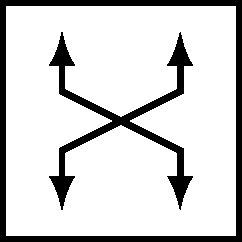
\includegraphics[width=0.9cm]{../common/fig-switch.pdf}
}
\providecommand{\router}{%
    
\includegraphics[width=0.9cm]{../common/fig-router.pdf}
}

% FIXME: scenario where 10.0.2.9 is machine A, then machine B
% FIXME: scenario where machine A and B both think they are 10.0.2.9
\begin{frame}[fragile]{}
\begin{tikzpicture}
\tikzset{
    computer/.style={inner sep=0mm,outer sep=0mm,execute at begin node={\computer}},
    computer alt/.style={inner sep=0mm,outer sep=0mm,execute at begin node={\computerAlt}},
    switch/.style={inner sep=0mm,outer sep=0mm,execute at begin node={\switch}},
    router/.style={inner sep=-1mm,outer sep=0mm,execute at begin node={\router},circle},
    connect/.style={draw,very thick,Latex-Latex},
    connect big/.style={draw,ultra thick,Latex-Latex},
    addr label/.style={align=left,font=\fontsize{9}{10}\selectfont\tt},
    arp table/.style={
        tight matrix,
        nodes={minimum height=.6cm},
        column 1/.style={nodes={text width=2.05cm,font=\small\tt}},
        column 2/.style={nodes={text width=1.75cm,font=\small\tt}},
        %row 1/.style={nodes={font=\small}},
    },
}
\begin{scope}[name prefix=first-]
    \node[computer,label={[addr label]north:MAC 77:\ldots:BB\\IP 10.0.2.2}] (n1-from) at (0, 0) {};
    \node[computer alt,label={[addr label]south:MAC 99:\ldots:BA\\IP 10.0.2.9}] (n1-to) at (0, -4) {};
    \node[switch] (sw) at (0, -2) {};
    \draw[connect] (n1-from) -- (sw);
    \draw[connect] (n1-to) -- (sw);
    \matrix[arp table,label={[label distance=0mm]north:.2's ARP table},inner sep=0mm,fill=white] 
        (arp table) at (2.75, -0.5) {
        10.0.2.9 \& 99:\ldots:BA \\
    };
\end{scope}
\begin{visibleenv}<2->
\draw[line width=2mm,black!50,dashed] (5.3, 2) -- ++(0, -8);
\begin{scope}[name prefix=second-,xshift=7cm]
    \node[computer,label={[addr label]north:MAC 77:\ldots:BB\\IP 10.0.2.2}] (n1-from) at (0, 0) {};
    \node[computer,label={[addr label]south:MAC \myemph<2>{CC:\ldots:01}\\IP 10.0.2.9}] (n1-to) at (2, -4) {};
    \node[switch] (sw) at (0, -2) {};
    \draw[connect] (n1-from) -- (sw);
    \draw[connect] (n1-to) -- (sw);
    \matrix[arp table,label={[label distance=0mm]north:.2's ARP table},inner sep=0mm,fill=white] 
        (arp table) at (2.75, -0.5) {
        10.0.2.9 \& |[alias=wrong mac box,alt=<2>{fill=red!10}]| 99:\ldots:BA \\
    };
    \begin{visibleenv}<2>
        \node[anchor=north,draw=red,very thick,align=left] at ([yshift=-.1cm]wrong mac box.south) {
            old entry prevents 10.0.2.2 \\
            from contacting new machine
        };
    \end{visibleenv}
\end{scope}
\node[anchor=south] at (2, 2) {Monday};
\node[anchor=south] at (8, 2) {Tuesday};
\end{visibleenv}
\end{tikzpicture}
\end{frame}

\begin{frame}{gratituous ARP requests}
    \begin{itemize}
    \item solution: send \textit{unsolicited} ARP messages
    \vspace{.5cm}
    \item CC:\ldots:01$\rightarrow$FF:\ldots:FF: request: who has 10.0.2.9, tell 10.0.2.9=CC:\ldots:01 
    \vspace{.5cm}
    \item<2-> request not reply b/c concerns about old/broken implementations
        \begin{itemize}
        \item ICMPv6 ND fixes this: \\
            message is `advertisement' ($\sim$ reply), not `solicitation' ($\sim$ request)
        \end{itemize}
    \end{itemize}
\end{frame}

\begin{frame}[fragile]{}
\begin{tikzpicture}
\tikzset{
    computer/.style={inner sep=0mm,outer sep=0mm,execute at begin node={\computer}},
    computer alt/.style={inner sep=0mm,outer sep=0mm,execute at begin node={\computerAlt}},
    switch/.style={inner sep=0mm,outer sep=0mm,execute at begin node={\switch}},
    router/.style={inner sep=-1mm,outer sep=0mm,execute at begin node={\router},circle},
    connect/.style={draw,very thick,Latex-Latex},
    connect big/.style={draw,ultra thick,Latex-Latex},
    addr label/.style={align=left,font=\fontsize{9}{10}\selectfont\tt},
    arp table/.style={
        tight matrix,
        nodes={minimum height=.6cm},
        column 1/.style={nodes={text width=2.05cm,font=\small\tt}},
        column 2/.style={nodes={text width=1.75cm,font=\small\tt}},
        %row 1/.style={nodes={font=\small}},
    },
}
\begin{scope}
    \node[computer,label={[addr label]north:MAC 77:\ldots:BB\\IP 10.0.2.2}] (n1-from) at (0, 0) {};
    \node[computer alt,label={[addr label]south:MAC 99:\ldots:BA\\IP \myemph<2>{10.0.2.9}}] (n1-toA) at (-2, -4) {};
    \node[computer alt,label={[addr label]south:MAC 09:\ldots:FE\\IP \myemph<2>{10.0.2.9}}] (n1-toB) at (2, -4) {};
    \node[switch] (sw) at (0, -2) {};
    \draw[connect] (n1-from) -- (sw);
    \draw[connect] (n1-toA) -- (sw);
    \draw[connect] (n1-toB) -- (sw);
\end{scope}
\end{tikzpicture}
\end{frame}

\begin{frame}{duplicate addresses}
    \begin{itemize}
    \item recommendations in RFC 5227 {\small ``IPv4 Address Conflict Detection''}
    \vspace{.5cm}
    \item probe for IP address before using it
        \begin{itemize}
        \item make sure to broadcast when starting to use address
        \item probably give up on address if conflict found
        \end{itemize}
    \item watch out for ARP messages indicating address in use
    \item on detecting conflict choose between:
        \begin{itemize}
        \item `defend' address with more gratituous requests
        \item give up address
        \end{itemize}
    \end{itemize}
\end{frame}


\subsection{ARP hijacking}

\usetikzlibrary{arrows.meta,calc,fit,matrix,shapes}
\providecommand{\computer}{%
    
\includegraphics[width=1cm]{../common/Noun_project_216.pdf}
}
\providecommand{\computerAlt}{%
    
\includegraphics[width=1cm]{../common/Noun_project_alt_cpu.pdf}
}
\providecommand{\switch}{%
    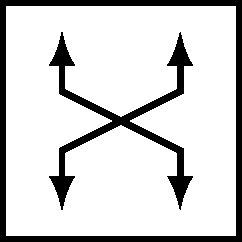
\includegraphics[width=0.9cm]{../common/fig-switch.pdf}
}
\providecommand{\router}{%
    
\includegraphics[width=0.9cm]{../common/fig-router.pdf}
}

\begin{frame}{ARP hijacking}
\begin{tikzpicture}
\tikzset{
    computer/.style={inner sep=0mm,outer sep=0mm,execute at begin node={\computer}},
    computer alt/.style={inner sep=0mm,outer sep=0mm,execute at begin node={\computerAlt}},
    switch/.style={inner sep=0mm,outer sep=0mm,execute at begin node={\switch}},
    router/.style={inner sep=-1mm,outer sep=0mm,execute at begin node={\router},circle},
    connect/.style={draw,very thick,Latex-Latex},
    connect big/.style={draw,ultra thick,Latex-Latex},
    addr label/.style={align=left,font=\fontsize{9}{10}\selectfont\tt},
    arp table/.style={
        tight matrix,
        nodes={minimum height=.6cm},
        column 1/.style={nodes={text width=2.05cm,font=\small\tt}},
        column 2/.style={nodes={text width=1.75cm,font=\small\tt}},
        %row 1/.style={nodes={font=\small}},
    },
    packet/.style={
        draw=blue,very thick,font=\tt\small,
        align=left,
    },
}
\begin{scope}
    \node[computer,label={[addr label]north:MAC 77:\ldots:BB\\IP 10.0.2.2}] (n1-from) at (0, 0) {};
    \node[computer alt,label={[addr label]south:MAC A5:\ldots:BA\\IP 10.0.2.9}] (n1-toA) at (-3, -4) {};
    \node[computer alt,label={[addr label]south:MAC 09:\ldots:FE},font=\Huge] (n1-toB) at (3, -4) {};
    \node[font=\huge] at (n1-toB) {\emoji{smiling-face-with-horns}};
    \node[switch] (sw) at (0, -2) {};
    \draw[connect] (n1-from) -- (sw);
    \draw[connect] (n1-toA) -- (sw);
    \draw[connect] (n1-toB) -- (sw);

    \begin{visibleenv}<2>
    \node[packet,anchor=north west] (blue spoof) at (3, 0) {
        09:\ldots:FE$\rightarrow$77:\ldots:BB \\
        10.0.2.9{\normalfont{} is }09:\ldots:FE
    };
    \node[packet,draw=violet,anchor=north west] (violet spoof) at (-1, -5) {
        09:\ldots:FE$\rightarrow$A5:\ldots:BA \\
        10.0.2.2{\normalfont{} is }09:\ldots:FE
    };
    \draw[blue,line width=1mm,dotted,-Latex] ([yshift=3mm]n1-toB.west) -- ([xshift=1mm]sw.center) -- (n1-from)
        coordinate[midway] (blue spoof point);
    \draw[violet,line width=1mm,dotted,-Latex] ([yshift=1mm]n1-toB.west) --
        ([xshift=-1mm,yshift=-1mm]sw.center) coordinate[midway] (violet spoof point) -- (n1-toA);
    \draw[blue,very thick] (blue spoof) -- (blue spoof point);
    \draw[violet,very thick] (violet spoof) -- (violet spoof point);
    \end{visibleenv}
    \begin{visibleenv}<3>
    \draw[Latex-Latex,red,line width=1mm] ([xshift=1mm]n1-from.south) -- ([xshift=1mm]sw.center)
        -- ([yshift=5mm]n1-toB.west);
    \draw[Latex-Latex,red,line width=1mm] ([yshift=-2mm]n1-toA.north east) -- ([yshift=-2mm]sw.center)
        -- ([yshift=0mm]n1-toB.west);
    \node[align=left,anchor=north west,draw=red,ultra thick] at (2, 0) {
        10.0.2.2 and 10.0.2.9 have \\
        ``poisoned'' ARP tables \\
        makes them send everything to attacker \\
        (instead of each other)
    };
    \end{visibleenv}
    % FIXME: ARP message to 10.0.2.2 with false 10.0.2.9
    % FIXME: ARP message to 10.0.2.9 with false 10.0.2.2
\end{scope}
\end{tikzpicture}
\end{frame}


\subsection{ARP/ND proxies}

\section{DHCP, SLAAC}



\section{backup slides}
\begin{frame}{backup slides}
\end{frame}

\end{document}
